\chapter[Stagnant Water Detection]{Stagnant Water Detection through Quadcopter}
Dengue~\cite{WHO15Dengue} is a troublesome debilating disease with no
known preventing vaccine, or cure. Doctors advocate that the best way
to avoid this disease is to avoid being bitten by mosquitoes which is
virtually an impossibility for many people in India.  The greatest
risk of contracting dengue (pronounced DENgee) is in the Indian
subcontinent.  

Technology is a must in tackling this situation.  The risk of disease
can be reduced by using insect repellents. In our institute, the
common method has been the spraying of insecticides.  Reports in the
media~\cite{china} indicate that China has flooded a small island
releasing half a million sterile mosquitoes to dominate the potent
mosquitoes. Such measures have unknown and unforeseen environmental
impact on the eco-system. Regardless, researchers are convinced that
there is no one single magic bullet to tackle the disease. 

Our work, started prior to the announcement of ``Project
Premonition,'' is similar to that of \cite{Microsoft15}.  Instead of
attempting to destroy the mosquito, we seek to detect the reason for
the increased outbreak, especially in urban areas.  Our work complements that
of \cite{Microsoft15} --- the goal in \cite{Microsoft15} is to ``catch wild
mosquitoes'' (typically in the outfield) by creating novel mosquito traps, and
then to test mosquitoes for pathogens. New traps are placed by drones, and
retrieved by drones. In contrast, we emphasize the need for
identifying the location of these traps.  

One of the major reasons behind the growth of mosquitoes is the
continuous existence of \emph{water puddles} around residencies in
urban India.  The virus is carried by mosquitoes, and these breed in
stagnant water. \emph{Can we detect stagnant water?}  When we surveyed
terraces (Fig.~\ref{fig:stagnantTeaser}) and ``chajjas'' of various buildings in
our institute, we found split AC air conditioners dumping condensed
water. Such areas can be surveyed using autonomous quadcopters.

\begin{figure}[h!]
\centering
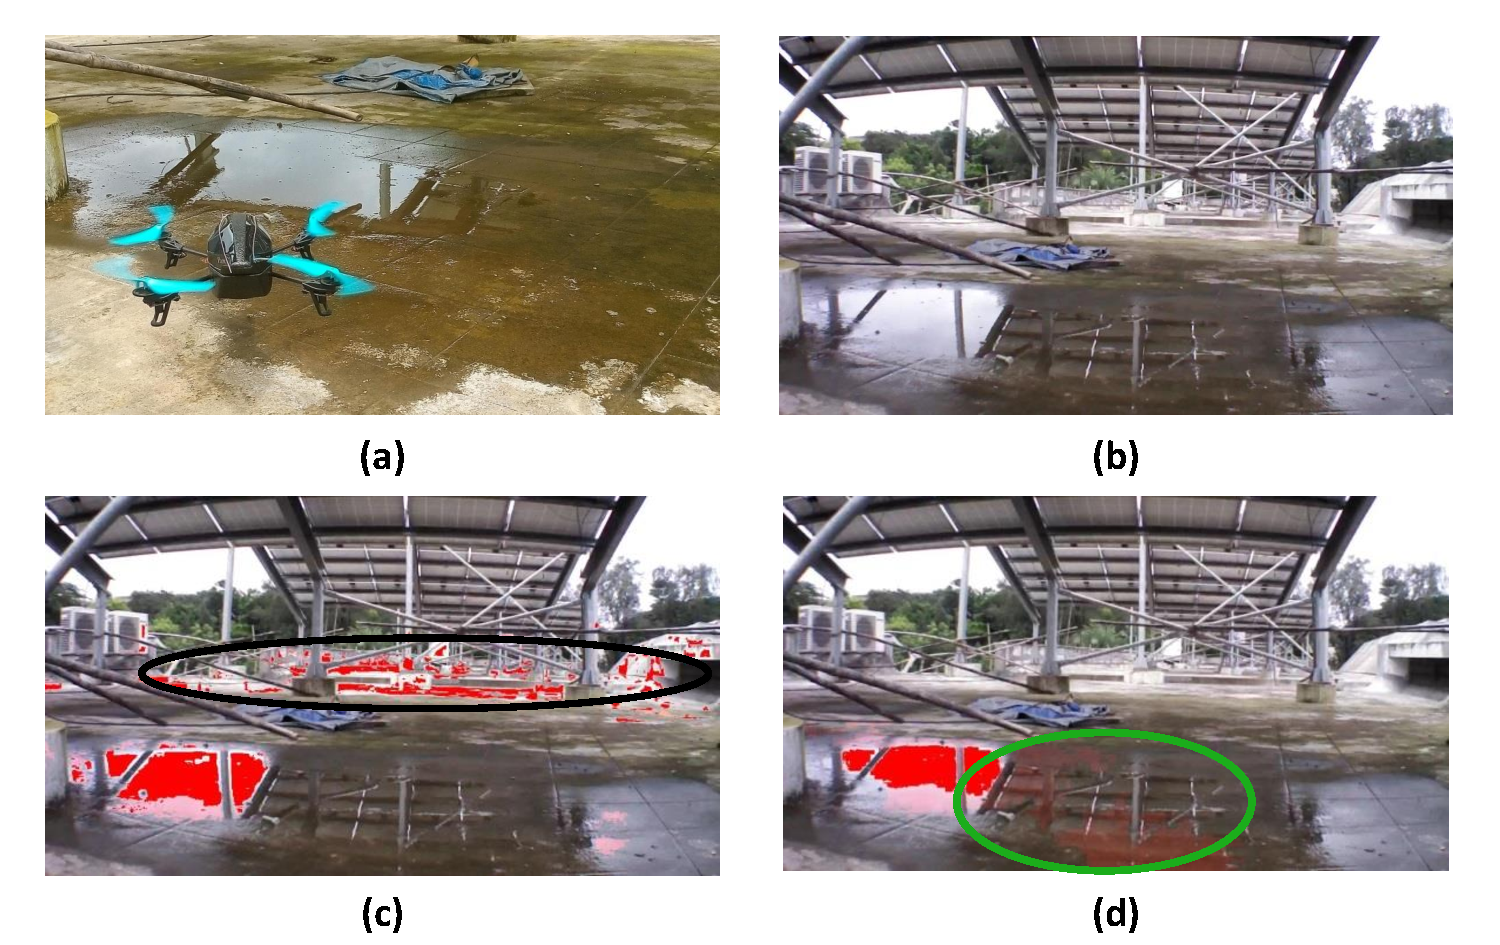
\includegraphics[width=\linewidth]{figures/stagnantWater/teaser.pdf}
\caption[Overview]{(a) Our hovering quadcopter (b) A
typical rooftop on campus (c) Earlier method \cite{rankin2004daytime} applied, and
  output marked in red (d) Our output. Notice (marked as black oval in
  (c)) that \cite{rankin2004daytime} confuses non-puddle patches as puddle.
  Also, note (marked as green ellipse in (d)) that \cite{rankin2004daytime} is
  not able to detect puddle which are dark.}
\label{fig:stagnantTeaser}  
\end{figure}

\textbf{Contributions:} The scientific challenge in identifying water
is that it is specular in nature, and acts like a mirror.  Water is
like a chameleon changing its color depending on the environment, and
there is no easy way of saying ``this is water'' based on its
appearance. In this work, we propose the use of an old paradigm of
optical flow for the novel application to stagnant water detection.
We couple it with a modern SVM-based method of classification.

\textbf{Related Work} The method in ~\cite{santana12} for detection of
water relies on the chaotic nature of water's dynamic texture to
exploit a measure of entropy over the trajectories obtained from
optical flow trackers over several frames. \cite{zhang10} has
introduced a descriptor which is tolerant to the flip transformation
and even non-rigid distortions, such as ripple effects.  \emph{These
  methods and others in the literature focus on the turbulent aspects
  of water}, largely absent in our application that focuses on
stagnant water.  Our method is closest to that of Rankin et
al.~\cite{rankin2004daytime, rankin11} who have implemented a rule-based water
detector based on sky reflections.  These rules are established
based on an analysis of images captured in wide-open areas on
cross-country terrain. Not only do we have new methods, \emph{our
datasets are captured in urban areas using a quadcopter and thus these
rules seem unlikely to be readily applicable.}

\section{Methodology}  Our method is based on a combination of color
based method with an optical flow based method.  We establish the
need for the combination in the first two subsections.

\subsection{Appearance-based Detection }

\begin{figure}[h!]
  \centering
  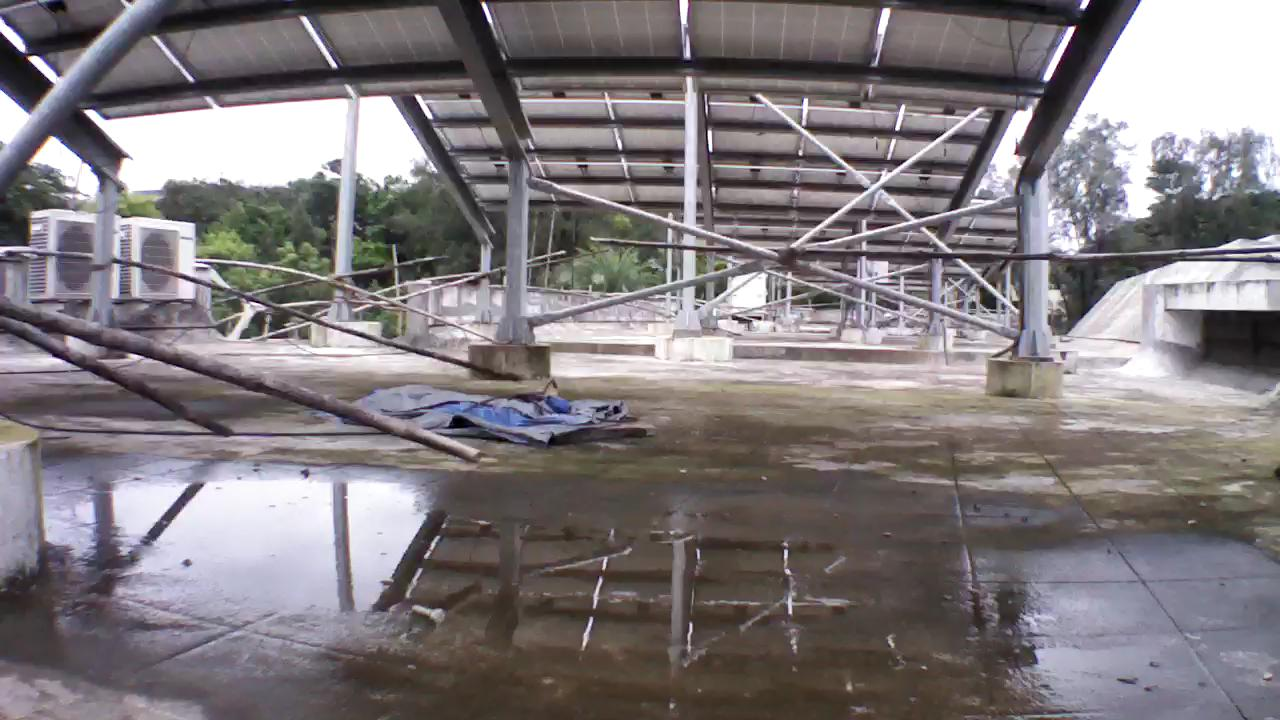
\includegraphics[width=0.4\linewidth]{figures/stagnantWater/IMG_PAIR_27_1.jpg} \hfill
  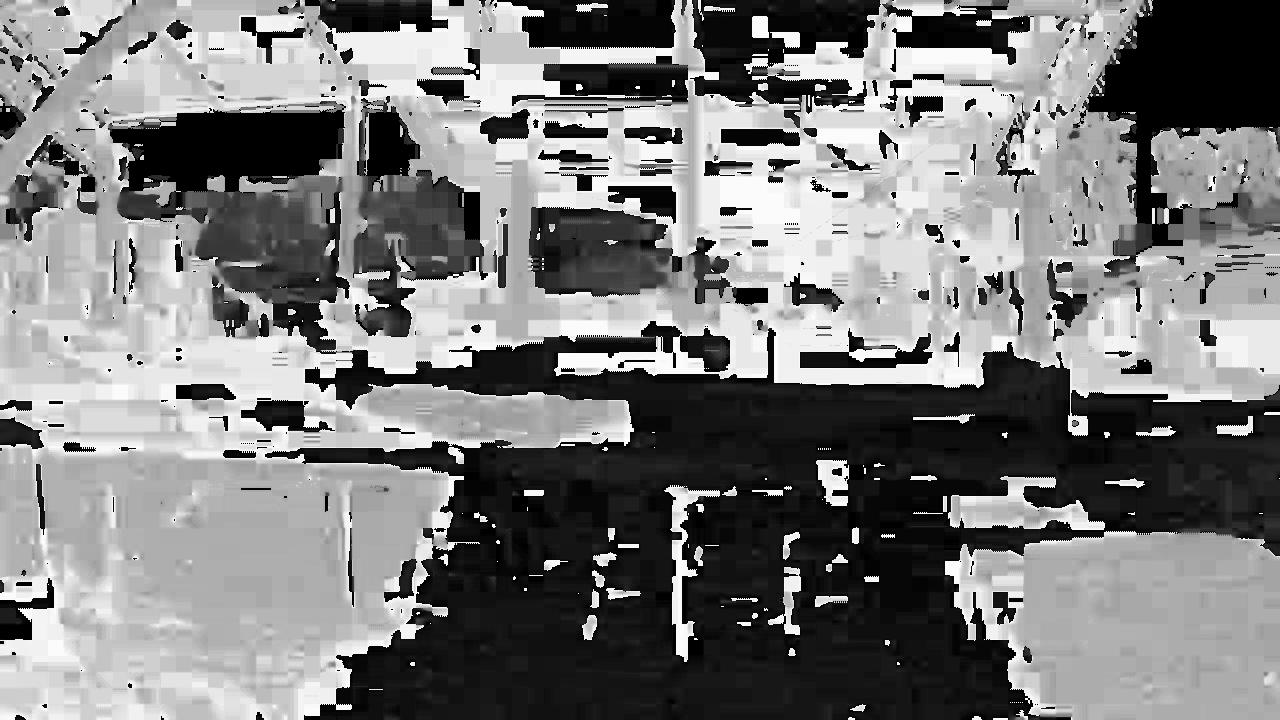
\includegraphics[width=0.4\linewidth]{figures/stagnantWater/IMG_PAIR_27_1_H.jpg} 

  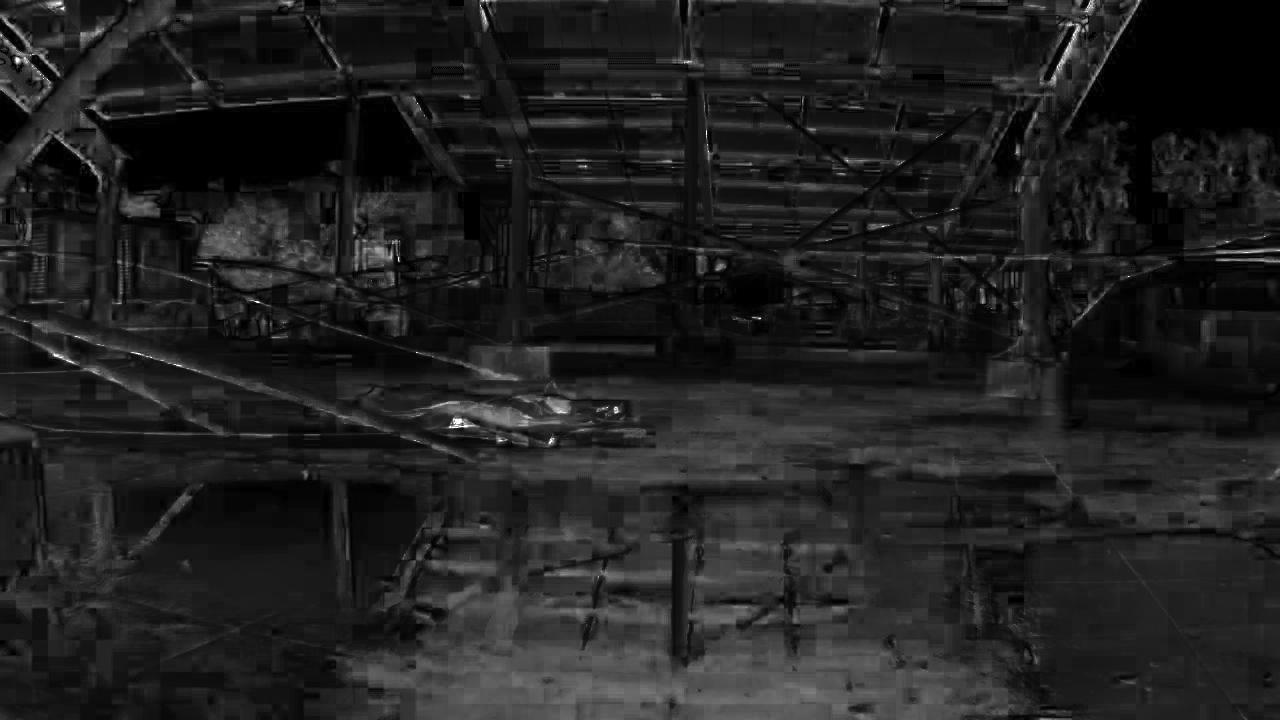
\includegraphics[width=0.4\linewidth]{figures/stagnantWater/IMG_PAIR_27_1_S.jpg} \hfill
  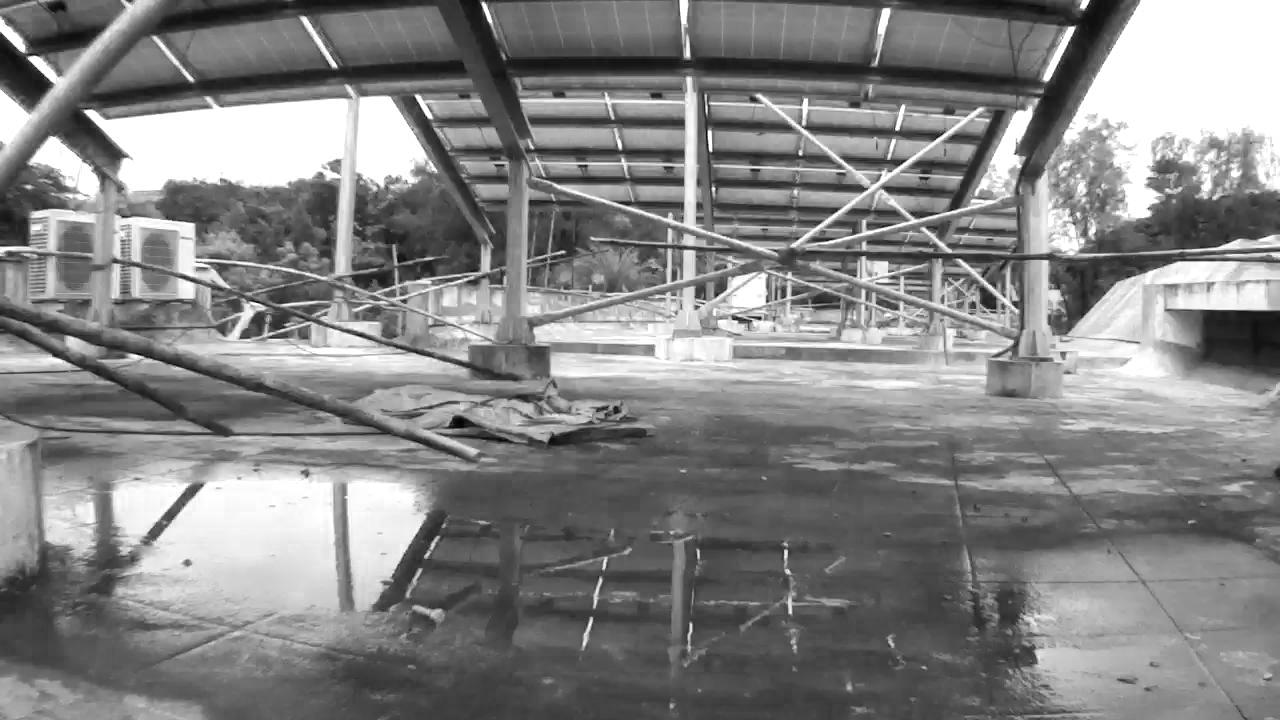
\includegraphics[width=0.4\linewidth]{figures/stagnantWater/IMG_PAIR_27_1_V.jpg}
  \caption[HSV Components]{An image (top left) and the HSV components.  The
  puddle has low saturation (bottom left) but high intensity (bottom right).
    The hue is indeterminable and is based on the environment.}
  \label{fig:HSV}
\end{figure}

Under ambient lighting conditions, puddle areas display high
brightness and low saturation as can be seen in
Fig.~\ref{fig:HSV}. Features based on these are fed to an SVM
classifier. Training an SVM is a labour intensive task.  To reduce the
effort, we have developed a tool shown in
Fig.~\ref{fig:training}. 
%This tool, and other data, will be released in the public domain.

% that
% capture this information locally could be used for puddle
% detection. Hence, considering a square image patch of small side
% dimension, $n$, a novel feature is used that performs the following
% steps:
% \begin{enumerate}
% \item Image is transformed from RGB color domain to HSV color space.
% \item Histogram for each channel having k bins is constructed
% \item The histogram values for three channels are concatenated to form a vector
% of length $3k$.
% \end{enumerate}
 
% Here, to capture sufficient statistics as well as constrain the feature size,
% number of bins, k = 64 is chosen, such that each bin contains 4 consecutive gray
% levels. Also, the side of square patch is taken as $n = 50$ to capture local
% characteristics.

% The given feature is used to train a Support Vector Machine(SVM) using a
% dataset of positively and negatively marked puddle patches. The
% positively-labelled as well as negatively-labelled patches are manually marked
% from a grid of size $m$ pixels overlaid on frames captured using quadcopter.
% Since RBF kernels have been useful to efficiently detect
% textures~\cite{Chapelle99}, it has been used for the given classifier. In our
% experiments, values of $m = 16$ is used.


% We have created a tool to select training data for the classifier. In this tool,
% image will be shown in grid fashion with block size of $50  \times 50$. 
% User will be enabled to draw contour over the desired region (puddle or
% non-puddle). The blocks enclosed by the contour will be selected. Additionally
% user may select additionally select blocks or deselect the selected blocks. The
% process is 

\begin{figure}[h!]
  \centering
  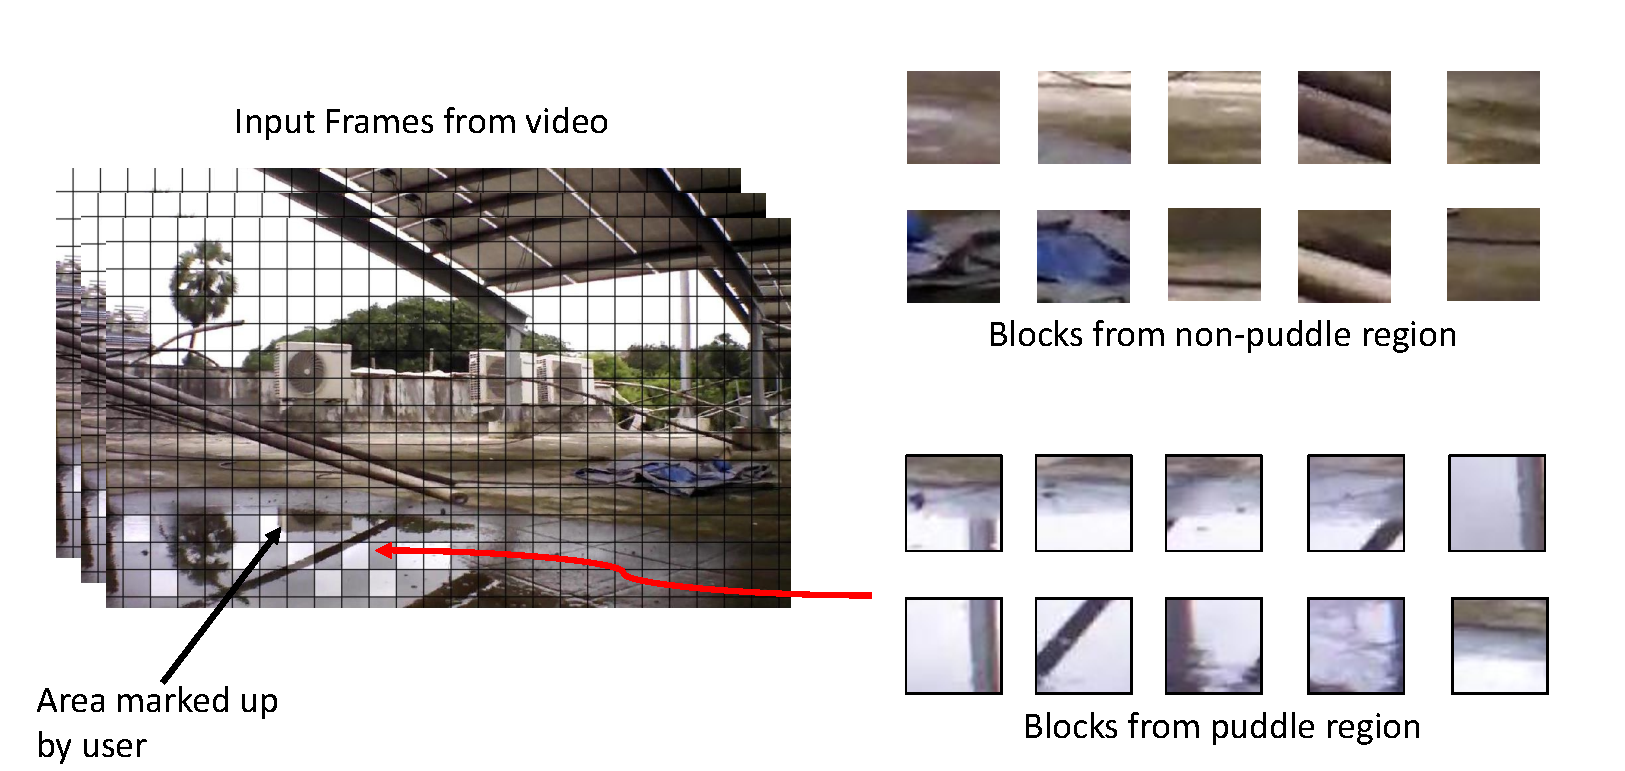
\includegraphics[width=0.9\linewidth]{figures/stagnantWater/trainingData.pdf}
  \caption[Creation of Training Data]{The process for creation of training data.
  The user selects the stagnant water area by drawing a contour to produce `positive'
    and `negative'  data.}
  \label{fig:training}
\end{figure}

\textbf{Failure of SVM-based methods:} The SVM detector is good at
detecting regions of sky reflected off a puddle.  In the HSV color
space, these regions have low saturation (S) and high brightness (V)
values, and are picked up with high reliability by the HSV histogram
feature based SVM detector. However, false negatives are also produced
since other reflected regions such as trees, buildings, etc. are
usually classified as non-puddle regions as many of these
characteristics is shared by negative images in the training data set.


\subsection{Optical flow based Detection}
Fortunately our images are captured by a moving quadcopter.  The
optical flow measures apparent motion of objects in a scene caused by
relative motion between camera and object. The magnitude of the
optical flow is high for objects that are close in comparison to
objects at a distance.  Fig.~\ref{fig:optical_flow} shows the
magnitude of optical flow calculated from two images.

\begin{figure}[h!]
  \centering
  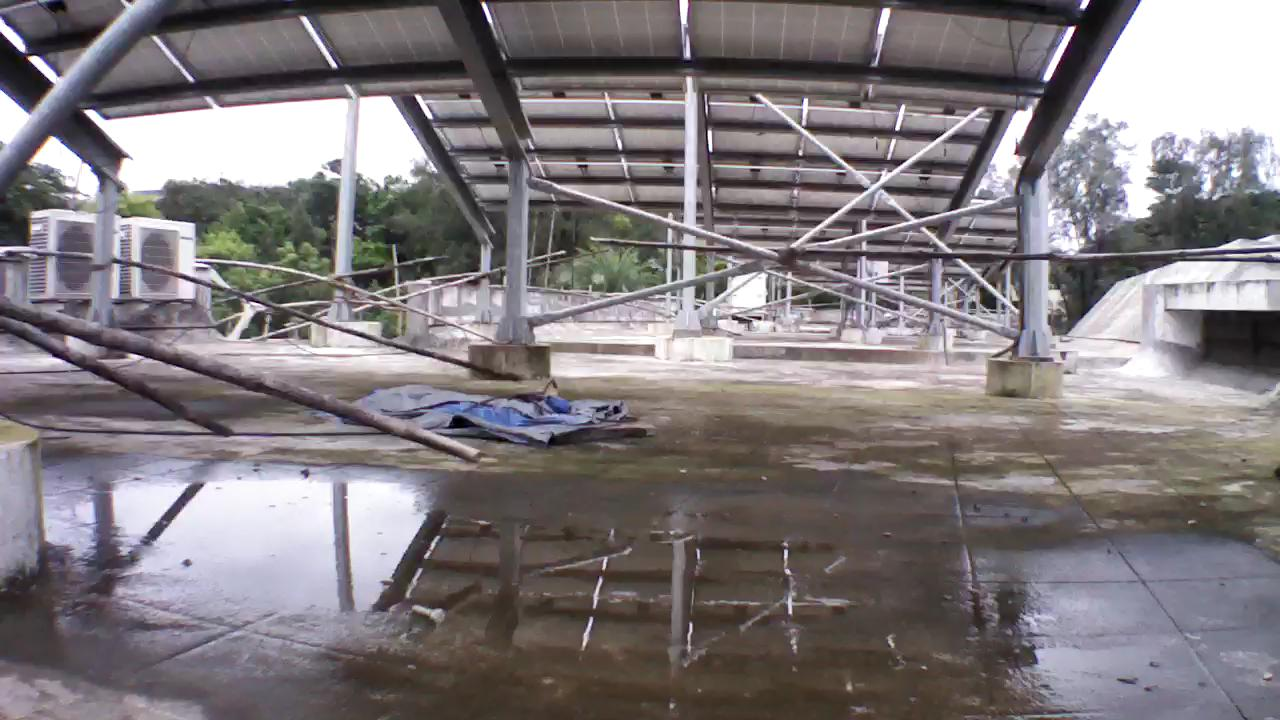
\includegraphics[width=0.32\linewidth]{figures/stagnantWater/IMG_PAIR_27_1.jpg} \hfill
  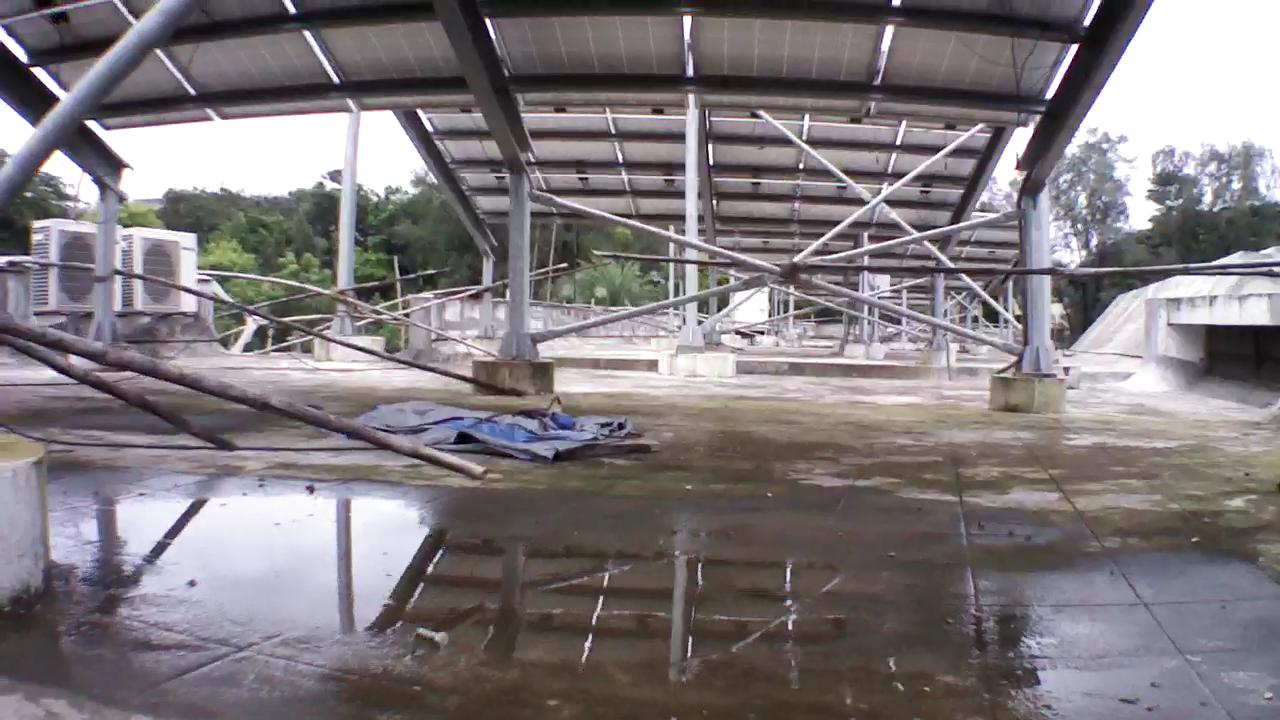
\includegraphics[width=0.32\linewidth]{figures/stagnantWater/IMG_PAIR_27_2.jpg} \hfill
  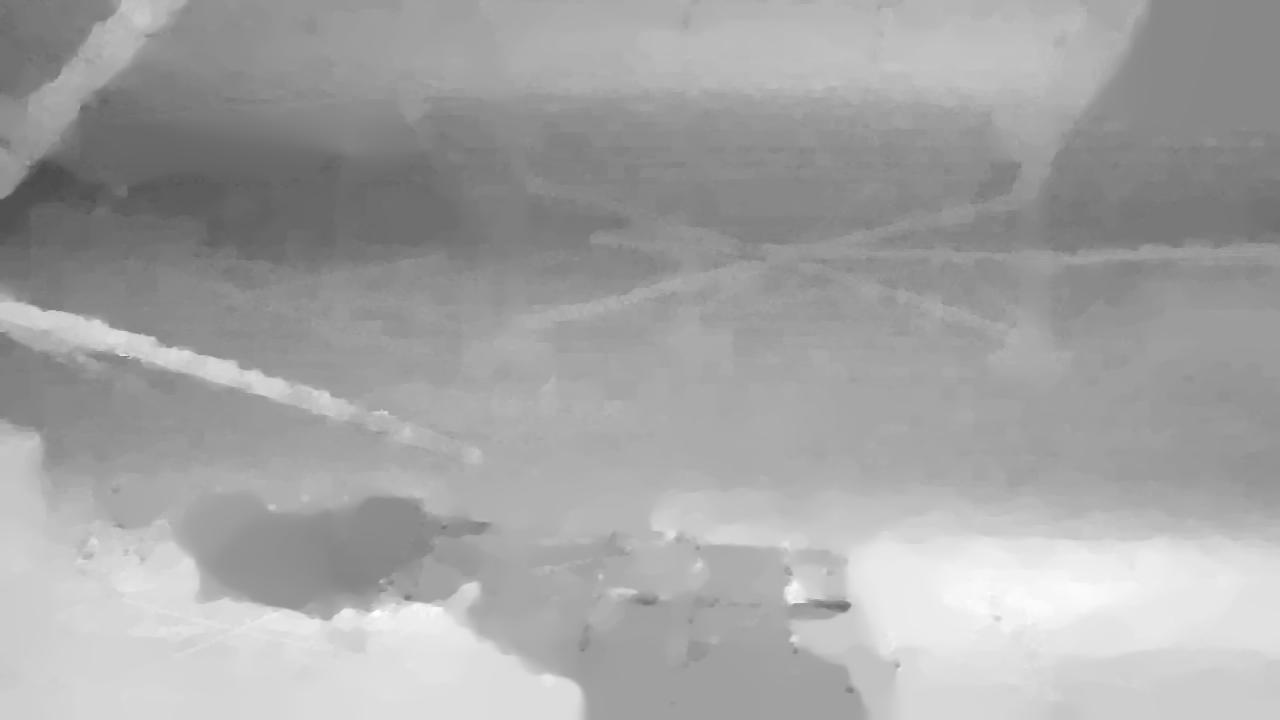
\includegraphics[width=0.32\linewidth]{figures/stagnantWater/IMG_PAIR_27_optical_flow.jpg}
  \caption[Sample Optical Flow]{Optical Flow. Left, Middle: Frames taken from
  positions which are $d$ units apart in 3D world. $ 0.01 \leq d \leq 0.1$. Right:
    Magnitude of optical flow. We observe that the magnitude of optical
    flow in the reflective parts of the puddle is relatively low.}
  \label{fig:optical_flow}
\end{figure}

A recent thesis \cite{Liu11Thesis} has one of the state of the art
algorithm for optical flow. One requirement is the need for
spatio-temporal smoothness constraint which can be challenging because
of the jerky movement of the UAV.  To resolve this, we use the
Inertial Measurement Unit (IMU) data available on the quadcopter to
synchronize positional information with the video sequence captured by
quadcopter. In short, we select the frame pair which are spatially the
closest, among a set of competing temporally adjacent frames.

\textbf{Failure of optical flow:} Optical flow is essentially being
used in a depth from parallax mode to exploit the fact that still
puddles behave like mirrors. The scenery reflected by such puddles is
usually at a much greater depth than the immediate surroundings of the
puddle.  Optical flow is largely independent of hue and saturation.
For the same reason, however, optical flow as a means of detecting
puddles will fail to report true positives when the object that is
being reflected is close by. In such cases, the saturation and
intensity values are useful.

Yet another reason for the failure for the optical flow is the
inability to distinguish true ``far away'' regions versus imagined far
away regions due to the mirror-like properties of water.  To handle
these false positives, we devise a horizon mask based on the principle
that water flows down.

\subsection{Combined approach}
\textbf{Horizon Mask:} The change in depth for far-away scenes as well
as their reflections on puddle, in consecutive frames, are hard to
distinguish. In previous work \cite{rankin11} such issues are avoided
by discarding a fixed-portion of image corresponding to far-off
regions, enforced by constrained input capture method. Due to
inapplicability of such constraints in the comparatively agile input
capture conditions of quadcopter, features derived from urban
environment are utilized for finding plausible puddle regions. In
urban setting, the high availability of structures in surroundings,
having distinctly flat surfaces and rectilinear silhouettes, enables
use of edge-detection based methods to bound planar regions that can
contain puddle. Applying the Hough transform with calibrated
parameters followed by length-based selection of lines detected, a
upper boundary for puddle region called `Horizon' is found. The
Horizon is in turn used to create a binary mask to be applied to local
scores from other techniques before normalization.


\begin{figure}[h!]
  \centering
  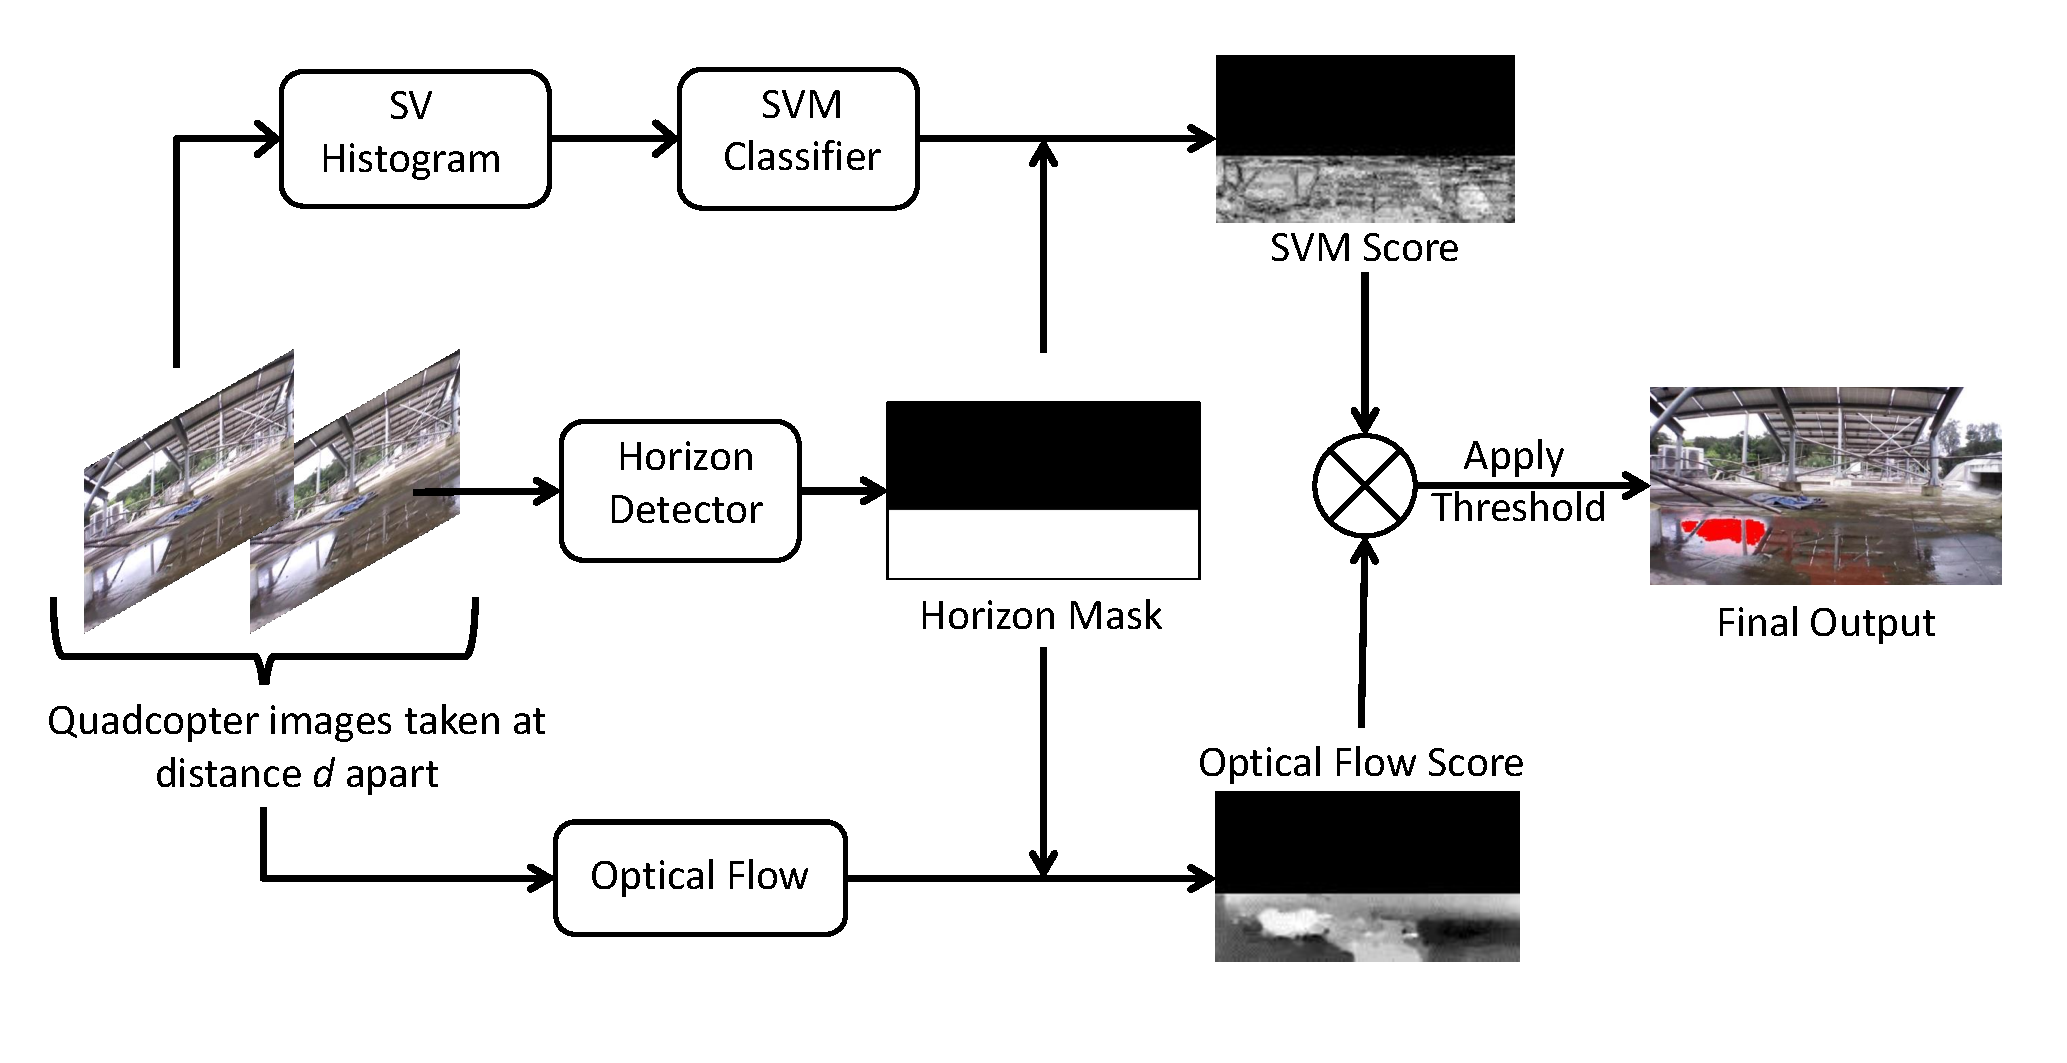
\includegraphics[width=0.9\linewidth]{figures/stagnantWater/overall_workflow.pdf}
  \caption{Overall architecture.}
  \label{fig:workflow}
\end{figure}

These observations suggested a novel combined approach as sketched
in Fig.~\ref{fig:workflow}.


% As illustrated in Figure~\ref{fig:workflow}, first we select coherent
% spatio temporal frames in pairs and obtain optical flow scores and
% SVM scores.  


% The SVM scores are obtained from classifier correspond to each patch of size, m
% ( m = 16 as mentioned in section), while for computational efficiency, optical
% flow is performed on frames downsampled to half of the original dimensions.
% But, to obtain a combined estimate based on both techniques, scores for a
% common patch size are necessary. Hence, the optical flow scores are divided
% into a grid of size $m/2$ pixels, each sub-patch of which are averaged to
% obtain the final optical flow score.

% The combined score obtained from optical flow and SVM classifier provides a
% probabilistic estimate of corresponding patch belonging a puddle. But, in order
% to include contribution towards the estimate based on neighborhood
% information, a sequence of morphological operations are applied on the
% combined score. From the resulting score, a mask denoting puddle region is
% obtained by thresholding based on statistical parameters.

\section{Experiments and Results}

All our experiments have been completed with the inexpensive consumer
quadcopter called Parrot's AR Drone. We remark that one should not
compare expensive military grade drones with such inexpensive drones.
For the purpose of showing the efficacy of this work, we also took a
picture of the scene from a distance with a 5 mega-pixel camera for
the reader to better understand the scene.  We covered urban places
such as terraces, constructions sites, building backyards,
pumping stations, and so on.  We have captured around eight different
types of datasets, each having around two-three minutes of video
(around 3000 frames each). 

%Due to page restriction, and file size
%restriction, in this paper, as well as in the
%supplementary material, we have shown only representative frames from
%captured videos. Frames not having any stagnant water are not shown. 
% Please see
% the supplementary material for additional results on remaining
% datasets as well as sample video captured through quadcopter.
% We have implemented our algorithm in Matlab R2014a. Experiments were performed
% on a PC with Intel Core i7 processor(@3.4GHz) and 8GB RAM.  
The source code is available at \cite{code} while the data sets we
created for this work can be downloaded from \cite{datasets}.

\textbf{Comparison:} We compare our method to \cite{rankin2004daytime} on
representative images since the methods in \cite{rankin11} do not apply. 
%See Fig.~\ref{fig:comparison}. 
It can be seen
from Fig.~\ref{fig:comparison} that in all images, \cite{rankin2004daytime} is
confusing bright patches as puddle patches (note red patches on walls, sky etc. in middle column in Fig.~\ref{fig:comparison}). Also, \cite{rankin2004daytime} is
not able to detect textured puddle images (as seen in the first row in
Fig.~\ref{fig:comparison}). (The confidence in detection is indicated by red hue in the output image. 
So, darker the red tinge, higher the confidence in detected water region. )
\begin{figure*}[p]
  \centering
  % \includegraphics[width=0.32\linewidth]{figures/stagnantWater/results/dataset_63full/IMG_PAIR_102_1} \hfill
  % \includegraphics[width=0.32\linewidth]{figures/stagnantWater/results/dataset_63full/output_102_jpl2} \hfill
  % \includegraphics[width=0.32\linewidth]{figures/stagnantWater/results/dataset_63full/output_102}
  
  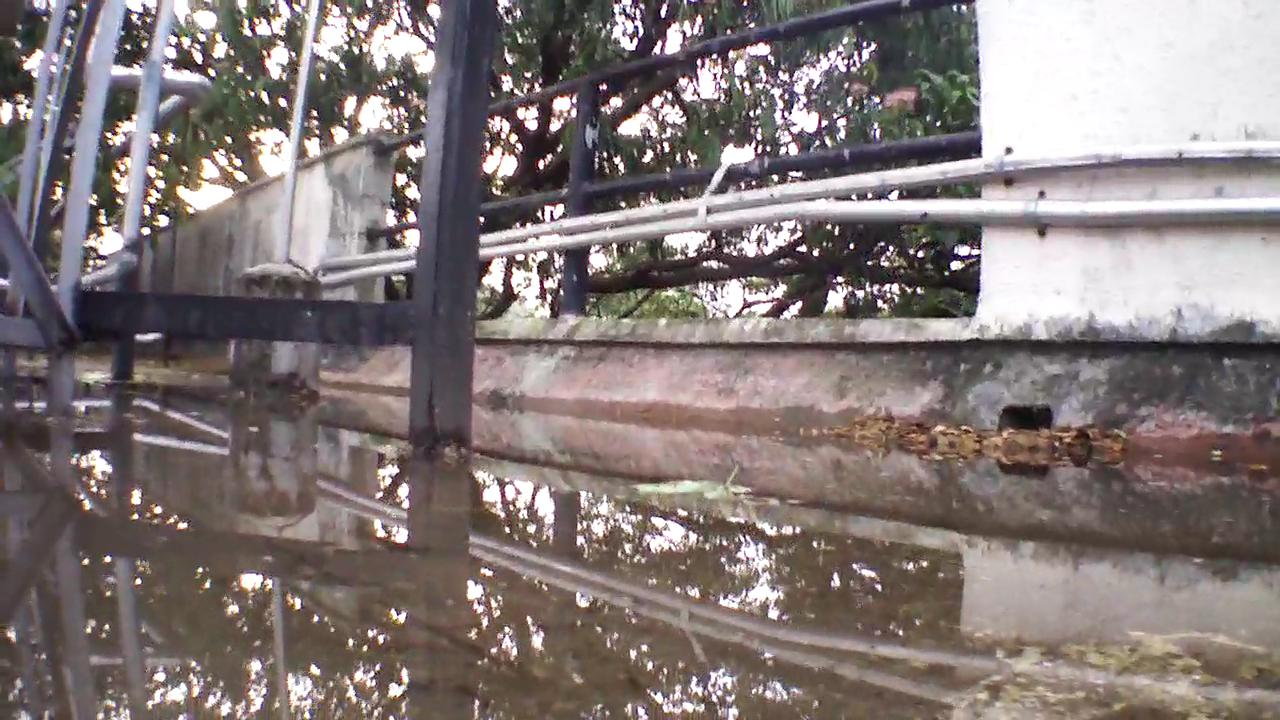
\includegraphics[width=0.32\linewidth]{figures/stagnantWater/results/dataset_73/IMG_PAIR_124_1.jpg} \hfill
  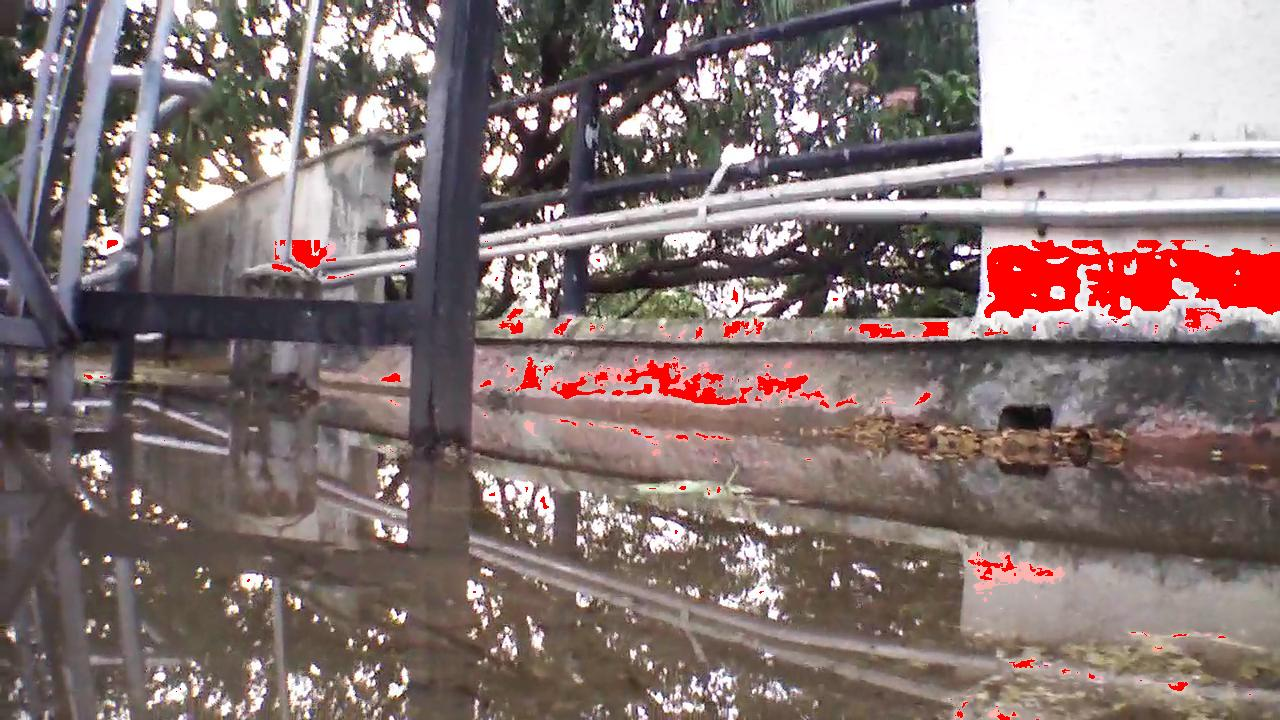
\includegraphics[width=0.32\linewidth]{figures/stagnantWater/results/dataset_73/output_124_jpl2.jpg} \hfill
  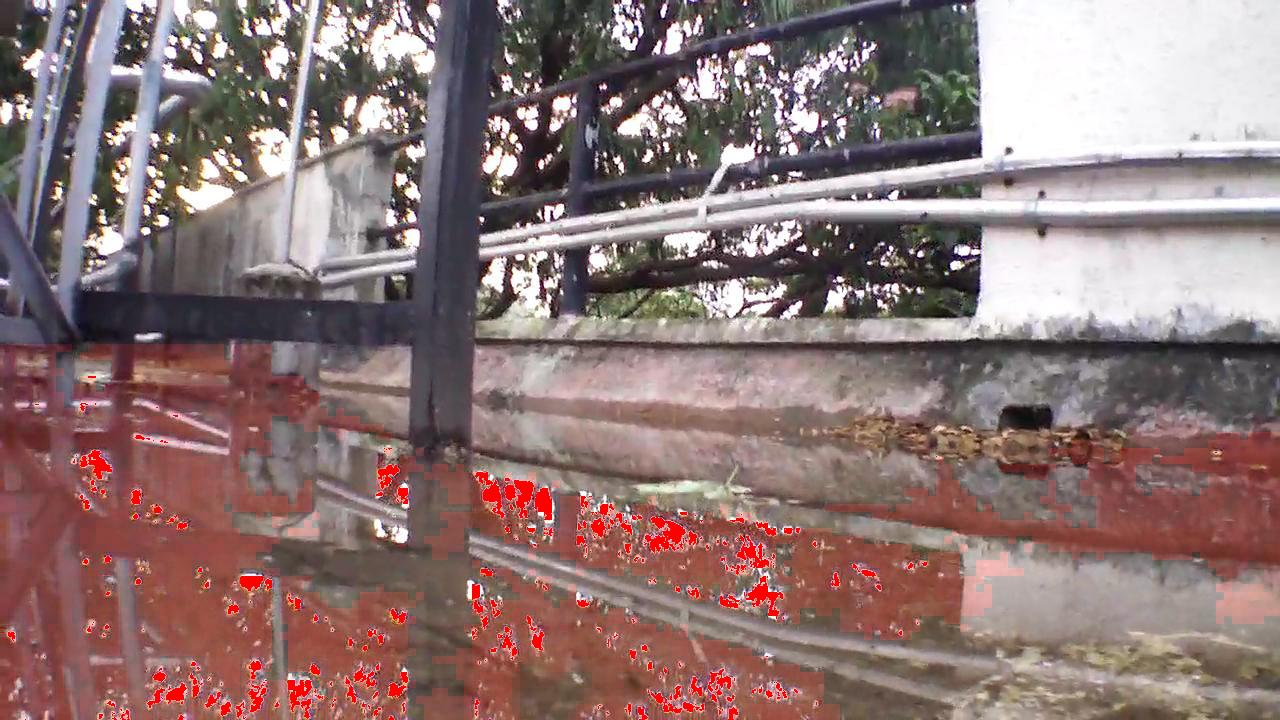
\includegraphics[width=0.32\linewidth]{figures/stagnantWater/results/dataset_73/output_124.jpg} \\
\medskip
  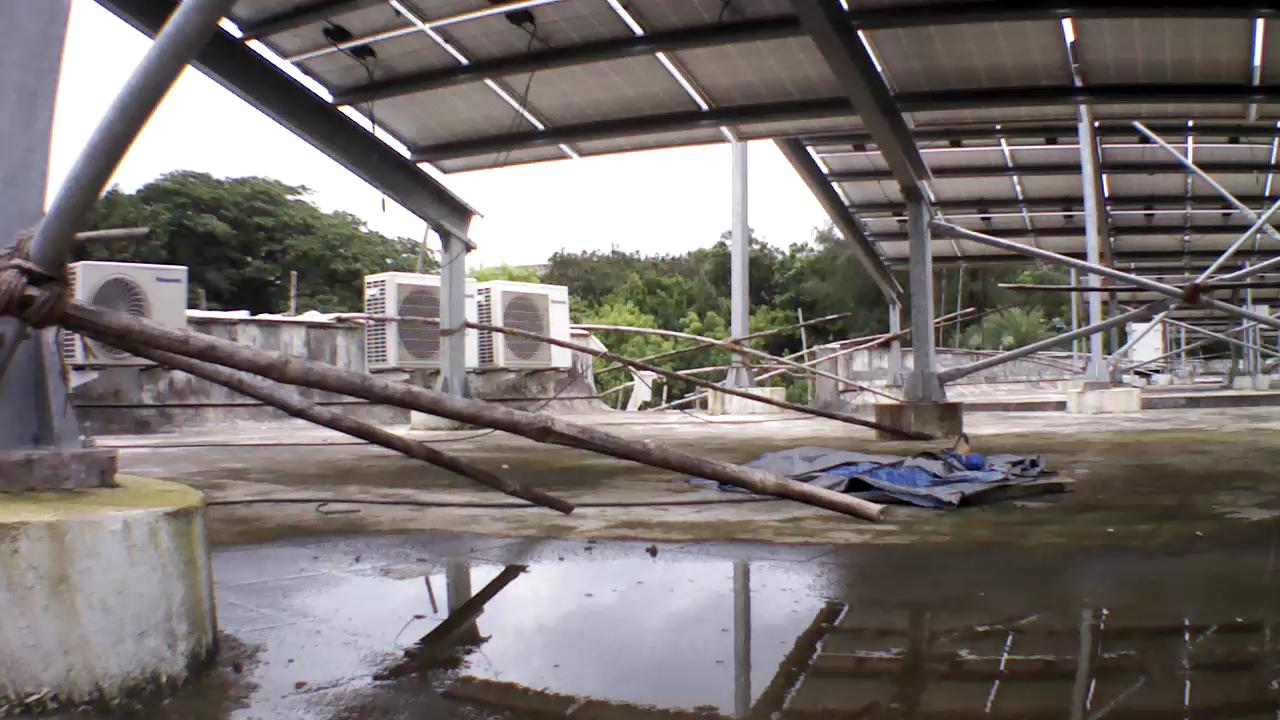
\includegraphics[width=0.32\linewidth]{figures/stagnantWater/results/dataset_81/IMG_PAIR_1_1.jpg} \hfill
  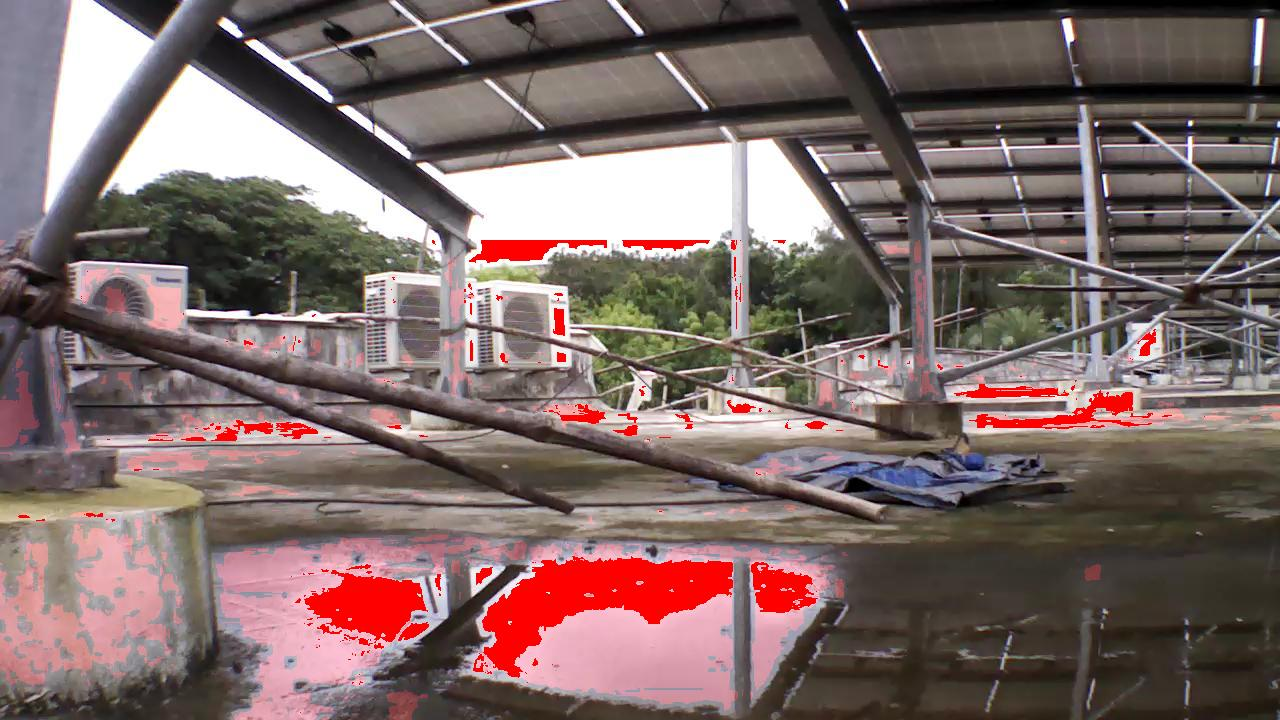
\includegraphics[width=0.32\linewidth]{figures/stagnantWater/results/dataset_81/output_1_jpl2.jpg} \hfill
  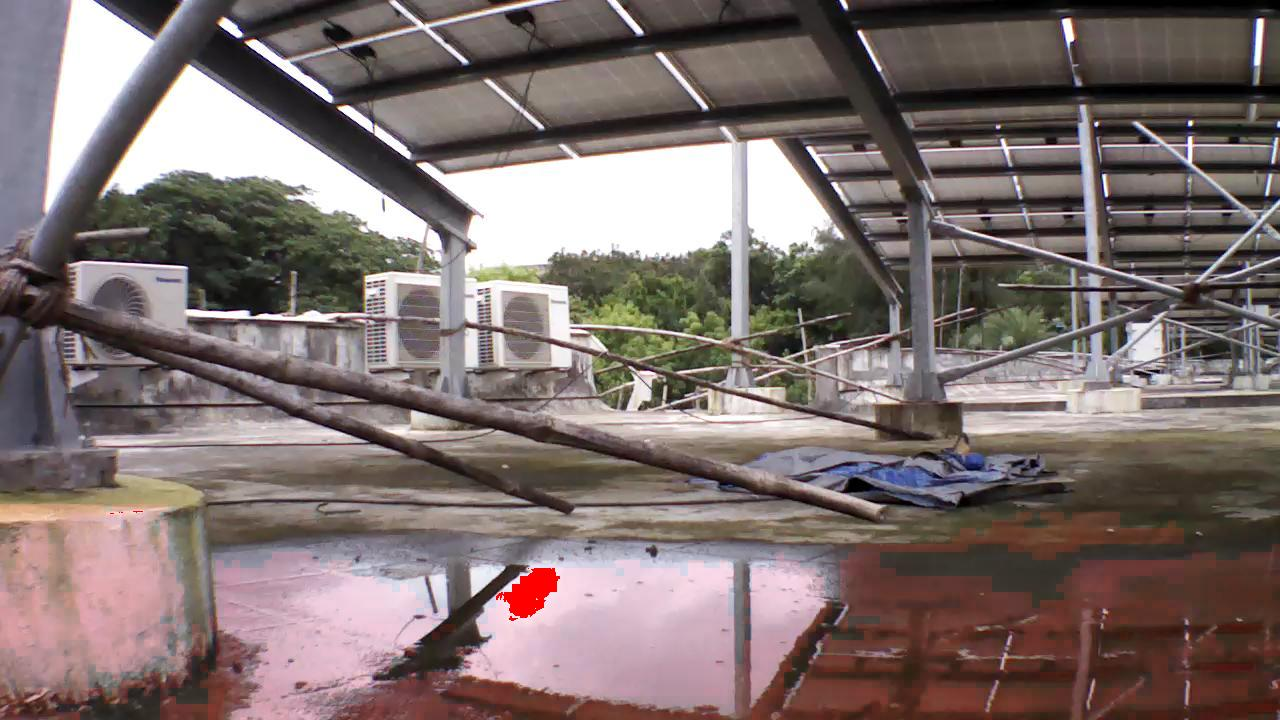
\includegraphics[width=0.32\linewidth]{figures/stagnantWater/results/dataset_81/output_1.jpg} \\
\medskip
  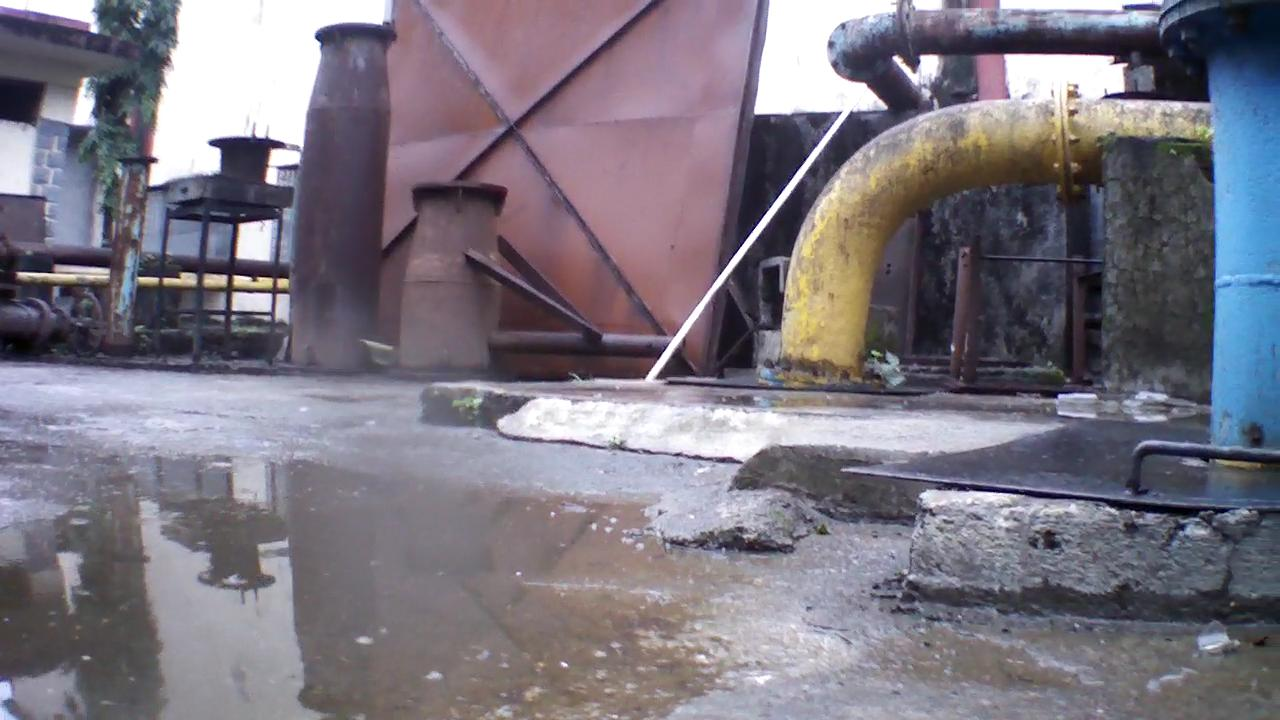
\includegraphics[width=0.32\linewidth]{figures/stagnantWater/results/dataset_82/IMG_PAIR_192_1.jpg} \hfill
  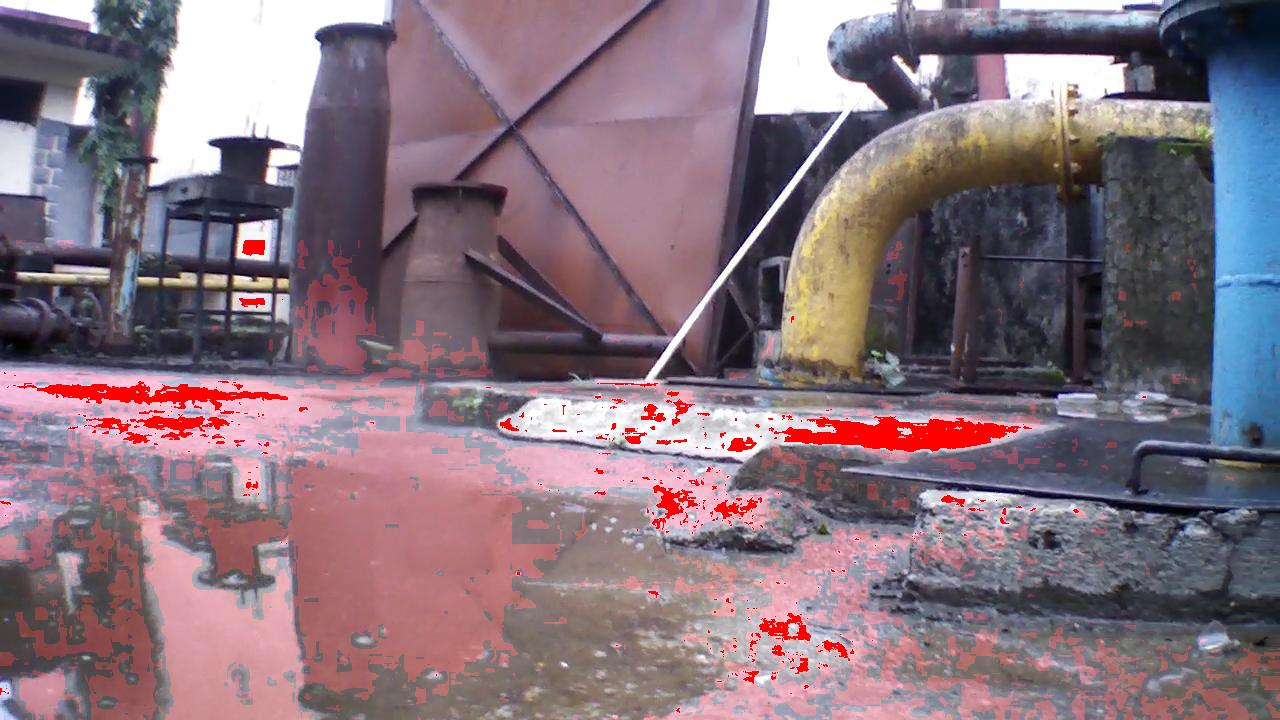
\includegraphics[width=0.32\linewidth]{figures/stagnantWater/results/dataset_82/output_192_jpl2.jpg} \hfill
  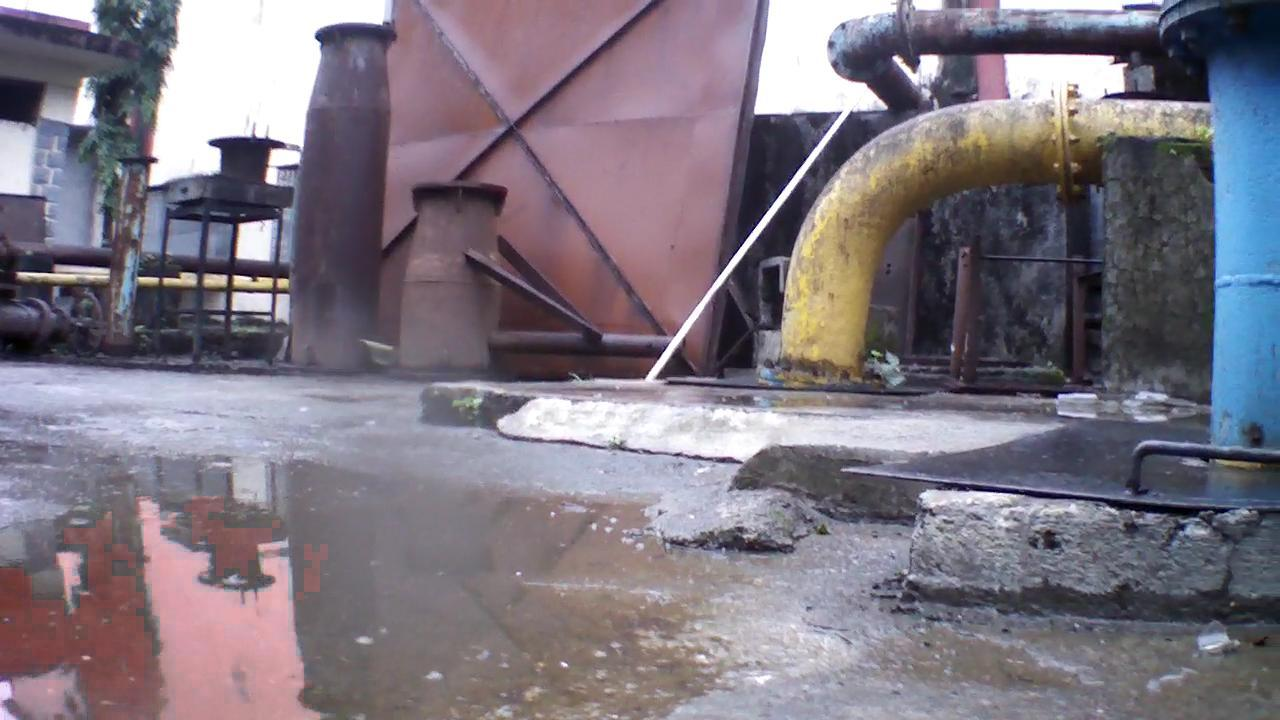
\includegraphics[width=0.32\linewidth]{figures/stagnantWater/results/dataset_82/output_192.jpg} \\
\medskip
  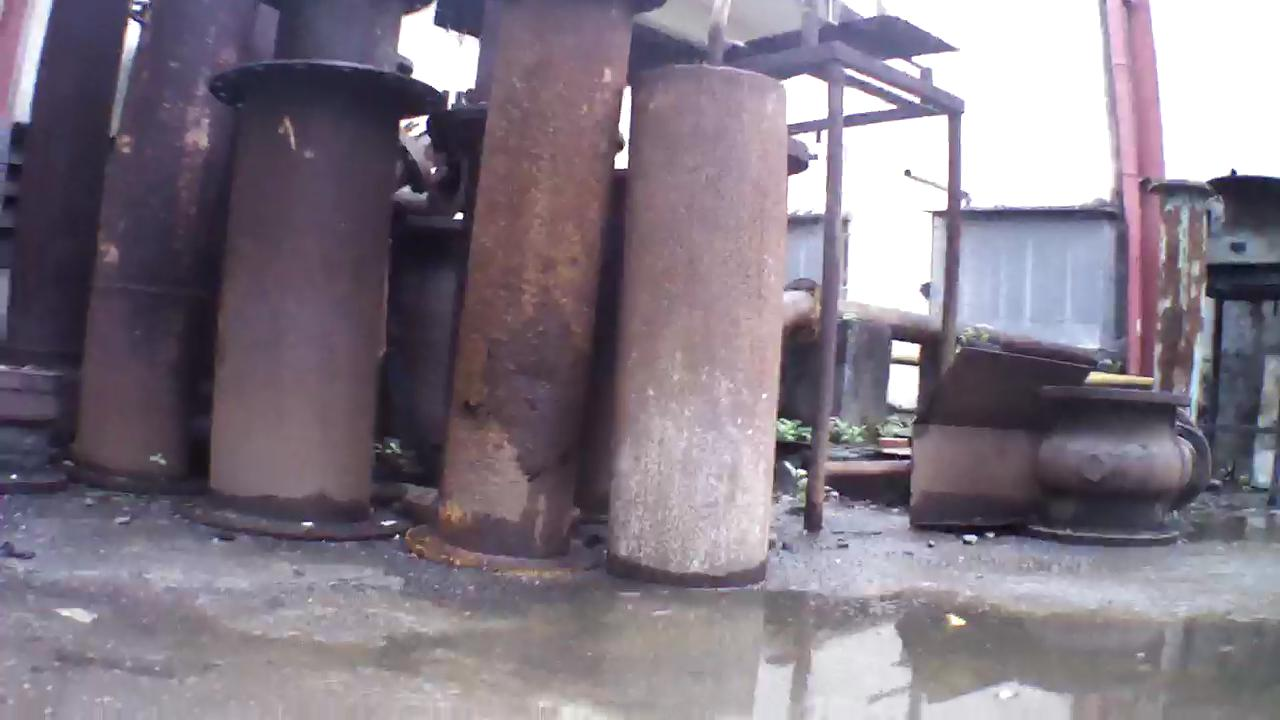
\includegraphics[width=0.32\linewidth]{figures/stagnantWater/results/dataset_83/IMG_PAIR_130_1.jpg} \hfill
  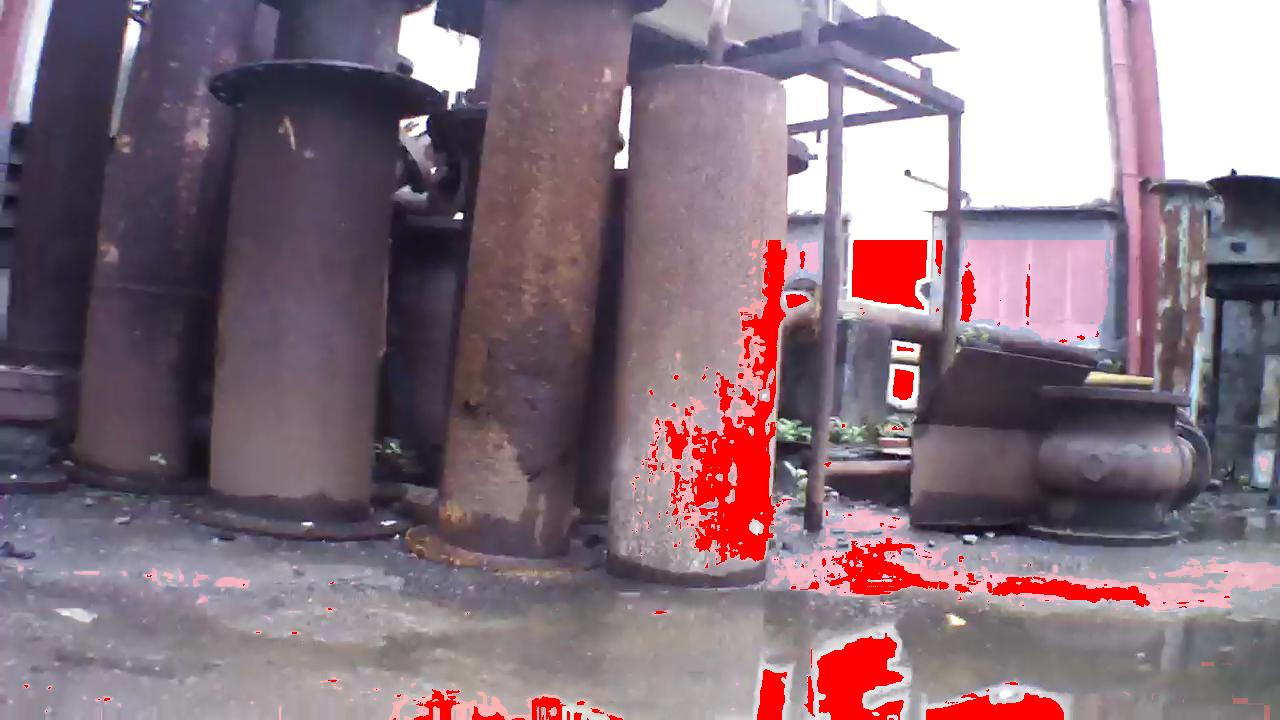
\includegraphics[width=0.32\linewidth]{figures/stagnantWater/results/dataset_83/output_130_jpl2.jpg} \hfill
  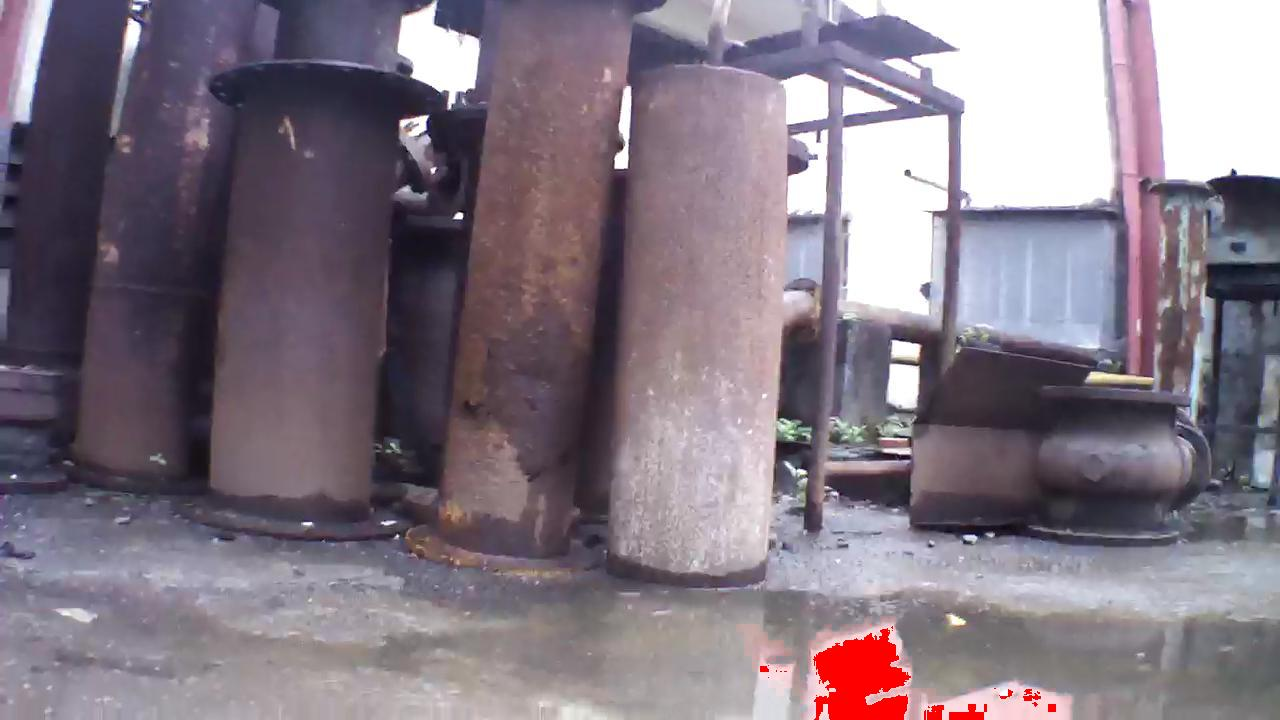
\includegraphics[width=0.32\linewidth]{figures/stagnantWater/results/dataset_83/output_130.jpg}
	
  \caption[Result Comparison]{Comparison of proposed method with
  \cite{rankin2004daytime}.
  Confidence in detection is indicated by red hue in the output image.
So, darker the red tinge, higher the confidence in detected water regions. \textbf{Left:} Original Image,
    \textbf{Middle:} Output of \cite{rankin2004daytime} \textbf{Right:}
    Proposed method. It can be seen that \cite{rankin2004daytime} is unable to
    detect textured puddle regions. Also, several false positives are
    seen to appear in the middle row.  Our method is sedate and
    sufficient to alert health workers.}
\label{fig:comparison}
\end{figure*}
 
\section{Conclusions}

Earlier in the introduction, we emphasized the need for detection of
stagnant water in hard to access areas. In the remaining parts of the
chapter we proposed a novel technique using a quadcopter.
The method proposed involved assigning a probabilistic measure to
image patches in input image frames, indicating likelihood of it being
a puddle. The measure was obtained by combining scores from an
SVM-based classifier, and an optical flow classifier. It is shown that
our approach produces better results in a variety of urban scenarios.

The main scientific contributions have been in addressing the specular
nature of water since water takes the color of its neighbourhood in a
puddle. Further an unmanned aerial vehicle can be quite jerky.  We
combined the IMU data on the quadcopter with the acquired imagery so
that the state of the art optical flow method can be used. 